\chapter{Suggestions to Improve the Existing System}

\section{System Perspective}
The purpose of the development of afetbilgi.com is mainly to help people who are affected
by disasters like earthquakes. To improved version of system context diagram can be seen in the Figure 4.1
\begin{figure}[H]
    \begin{center}
        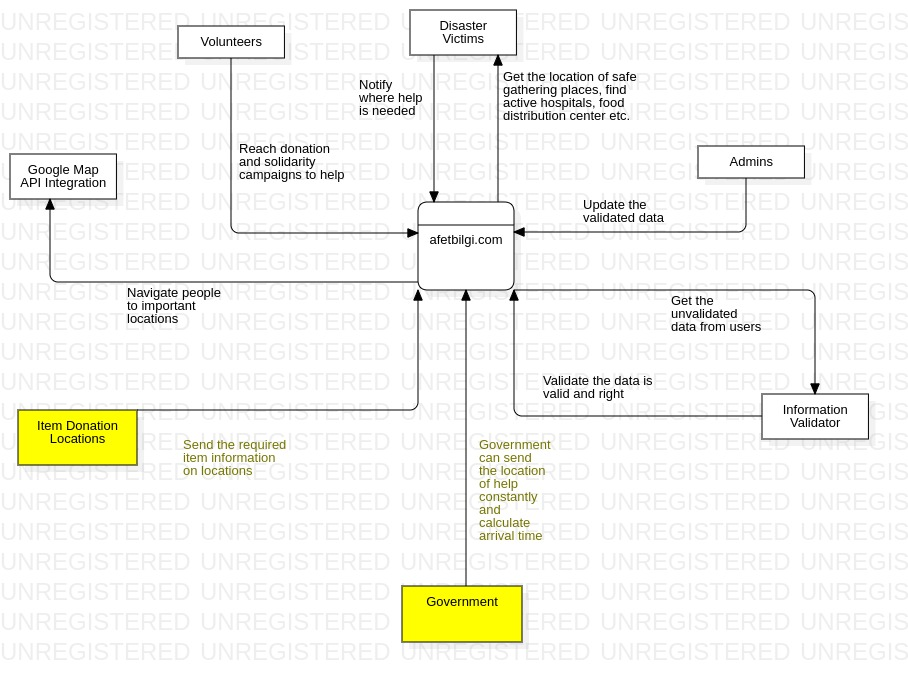
\includegraphics[scale = 0.50]{assets/System Context DiagramSuggestion.jpg}
        \caption[Suggested System Context Diagram]{Suggested System Context Diagram}
    \end{center}
\end{figure}
\subsection*{System Interfaces}
In addition to System Inferfaces explained in Section 1.3.1.1, it can included the Notification System and Email Sending Integration.

\begin{itemize}
    \item \textbf{Notification System: } This system will allow afetbilgi.com that user who are in the disaster area can be informed by any emergency situation by opening the notifications.
    \item \textbf{Email Sending System: } This system will allow users to get the crucial information for the city they need by email. It works similar to PDF integration of the system however by email, it can allow getting information by automatically, not opening the website. 
\end{itemize}

\subsection*{User Interfaces}
The mobile application of the project can be done. The less digital knowledgeable people can adapt themselves to use the application.
Because elderly people may find the hard to write afetbilgi.com to search button instead of clicking the application icon. 

\subsection*{Hardware Interfaces}
The hardware requirements is the same with the original version of afetbilgi.com.

\subsection*{Software Interfaces}
\begin{itemize}
    \item \textbf{Database: } The system will hold a lot of different data. As a result, more complex database can be implemented to the system.
    \item \textbf{Operating System: } The system can be adapted to the mobile application as well. Therefore addition to internet browser, the application can be developed for Google Play Store and App Store.
\end{itemize}

\subsection*{Memory Constarints}
There is no issue with memory constraints in the system.

\subsection*{Operations}
The operations may be provided in the future by afetbilgi.com can be partitioned into:

\textbf{User operations: }

\begin{itemize}
    \item Reaching important resources
    \item Seeing Location of Healthcare Services
    \item Reaching other websites to help victims
    \item Seeing contact info and location places associated with general needings
    \item Filters the info by cities
    \item Seeing data of website on a Map
    \item Contacting with Developers and Maintainters
    \item \textcolor{yellow}{Seeing live location of the donation and helps}
    \item \textcolor{yellow}{Learning required supplu amount for item donating locations}
    \item \textcolor{yellow}{Seeing hospital occupancy rate}
\end{itemize}

\textbf{Admin operations: }
\begin{itemize}
    \item Validate the information
    \item Update the information
\end{itemize}

\textbf{System Operations: }
\begin{itemize}
    \item Creating a PDF document which includes info
    \item Multi Language Support
    \item \textcolor{yellow}{Sending information mail which includes info}
    \item \textcolor{yellow}{Sending notification to user in emergencies}
\end{itemize}

\section{External Interfaces}

\begin{figure}[H]
    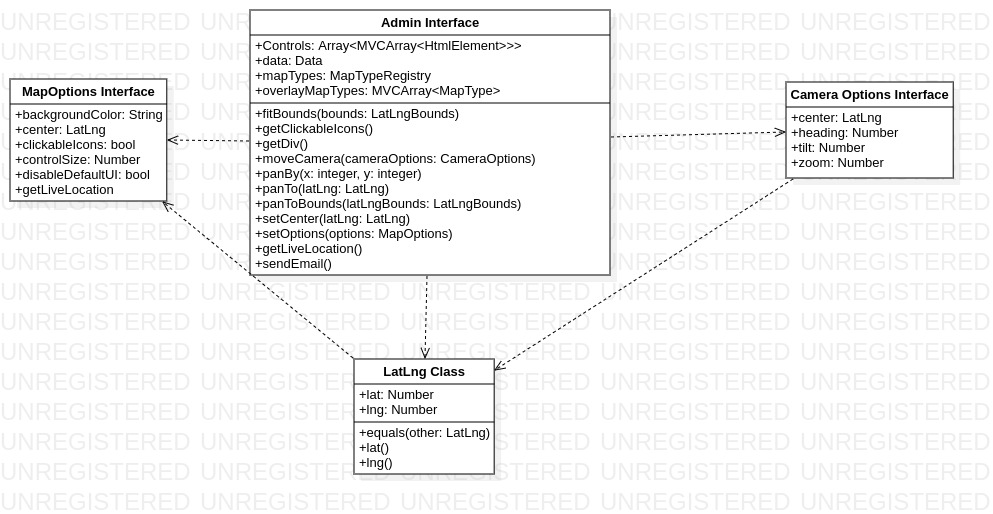
\includegraphics[scale = 0.4]{assets/externalSuggestion.jpg}
    \caption[External Interfaces for afetbilgi.com]{External Interfaces for afetbilgi.com}
\end{figure}

\section{Functions}

\begin{figure}[H]
    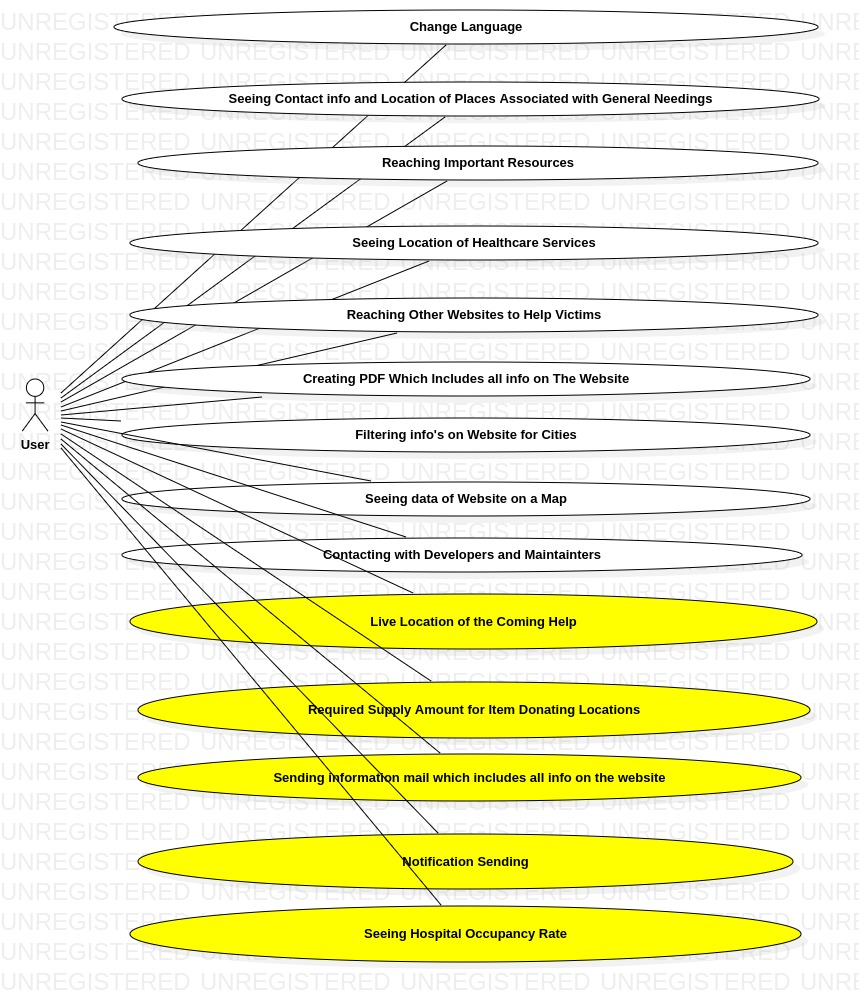
\includegraphics[scale = 0.5  ]{assets/UseCaseDiagramSuggestion.jpg}
    \caption[Use Case Diagram]{Use Case Diagram}
\end{figure}

\begin{center}
    \begin{table}[H]
        \begin{tabular}{| m{3cm}| m{10cm} |}
            \hline
            \textbf{Use case name} & Live Location of the Coming Help\\
            \hline
            \textbf{Actors} & Volunteers, User\\
            \hline
            \textbf{Description} & When volunteers send a supply for the victims, victims can see the supplies live location and the estimation time to arrival provided by the officials. As a result, they can prepare themselves accordingly.\\
            \hline
            \textbf{Data} & Current Location\\
            \hline
            \textbf{Preconditions} & - \\
            \hline
            \textbf{Stimulus} & Users tries to find supply and their estimation arrival time.\\
            \hline
            \textbf{Basic flow} & Step 1 - User clicks map to open map from main page.\\
                                & Step 2 - User finds the desired location from map. \\
                                & Step 3 - User clicks the supply location to get the information about estimation arrival time. \\
            \hline
            \textbf{Alternative flow} & - \\
            \hline
            \textbf{Exception flow} & If an error occurs on map side, google map API throws an error.\\
            \hline
            \textbf{Postconditions} & - \\
            \hline
        \end{tabular}
        \caption[Live Location of the Coming Help]{Live Location of the Coming Help}
    \end{table}
\end{center}

\begin{figure}[H]
    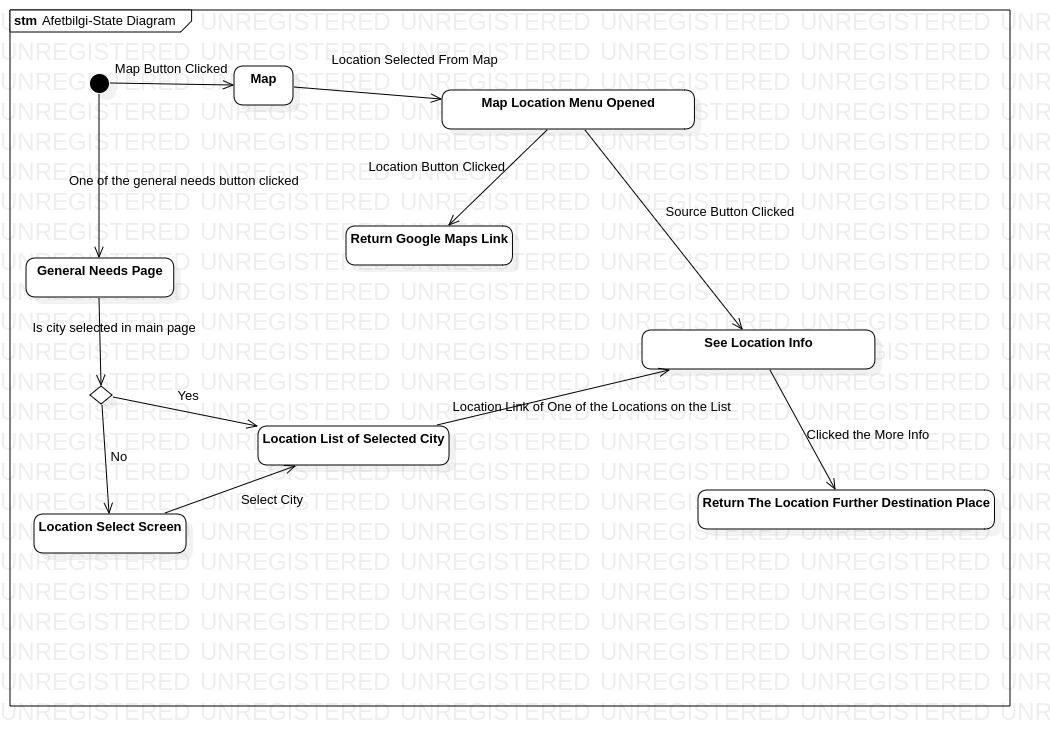
\includegraphics[scale = 0.45]{assets/StateDiagramSuggestion.jpg}
    \caption[State Diagram for Live Location of Help]{State Diagram for Live Location of Help}
\end{figure}

\begin{center}
    \begin{table}[H]
        \begin{tabular}{| m{3cm}| m{10cm} |}
            \hline
            \textbf{Use case name} & Required Supply Amount for Item Donating Locations\\
            \hline
            \textbf{Actors} & Volunteers\\
            \hline
            \textbf{Description} & Volunteers can collect the required items faster with this function.\\
            \hline
            \textbf{Data} & Selected city\\
            \hline
            \textbf{Preconditions} & - \\
            \hline
            \textbf{Stimulus} & Users tries to find required supplies for their helps.\\
            \hline
            \textbf{Basic flow} & Step 1 - User clicks one of the button which is a donation button on the main page.\\
                                & Step 2 - User finds the supply location from map. \\
                                & Step 3 - User clicks the supply location to get the information about required items. \\
            \hline
            \textbf{Alternative flow} & - \\
            \hline
            \textbf{Exception flow} & If there is not any required items, it throws an message.\\
            \hline
            \textbf{Postconditions} & - \\
            \hline
        \end{tabular}
        \caption[Required Supply Amount for Item Donating Locations]{Required Supply Amount for Item Donating Locations}
    \end{table}
\end{center}

\begin{center}
    \begin{table}[H]
        \begin{tabular}{| m{3cm}| m{10cm} |}
            \hline
            \textbf{Use case name} & Sending information mail which includes all info on the website\\
            \hline
            \textbf{Actors} & User\\
            \hline
            \textbf{Description} & User can send a email containing the information on website to reach the info offline, or any other purpose.\\
            \hline
            \textbf{Data} & Selected city. (If there is one).\\
            \hline
            \textbf{Preconditions} & - \\
            \hline
            \textbf{Stimulus} & User tries to get all information of website.\\
            \hline
            \textbf{Basic flow} & Step 1 - User clicks send information by email button.\\
                                & Step 2 - Write your email address to the text area. \\
                                & Step 3 - Site returns a preformed email containing all information about the city (if selected) selected by the user, in the selected language. \\
            \hline
            \textbf{Alternative flow} & - \\
            \hline
            \textbf{Exception flow} & - \\
            \hline
            \textbf{Postconditions} & - \\
            \hline
        \end{tabular}
        \caption[Sending Information Email]{Sending Information Email}
    \end{table}
\end{center}

\begin{figure}[H]
    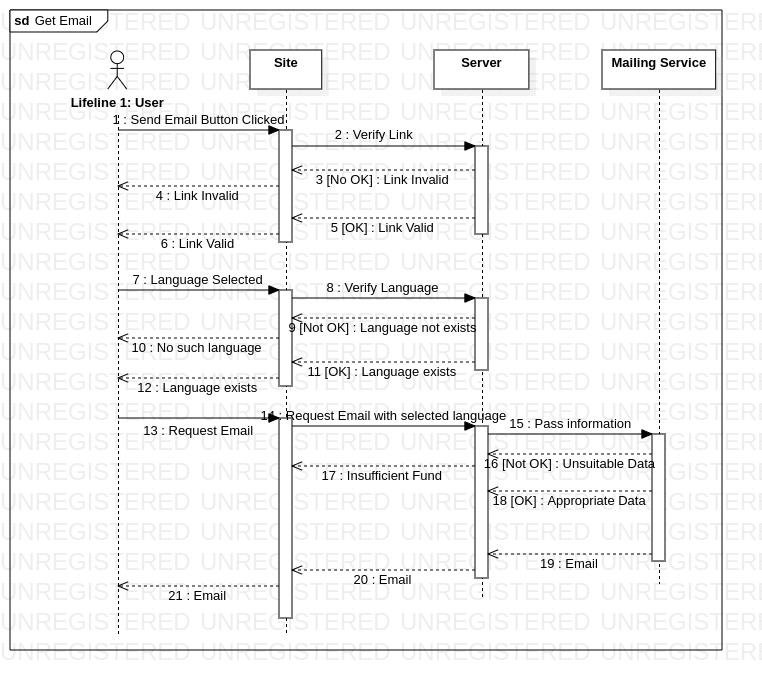
\includegraphics[scale = 0.6]{assets/SequenceDiagramSuggestion.jpg}
    \caption[Sending Email Sequence Diagram]{Sending Email Sequence Diagram}
\end{figure}

\begin{center}
    \begin{table}[H]
        \begin{tabular}{| m{3cm}| m{10cm} |}
            \hline
            \textbf{Use case name} & Notification Sending\\
            \hline
            \textbf{Actors} & User\\
            \hline
            \textbf{Description} & User can open notifications. By opening the notification system, system send user to warning about any occuring disaster like tsunami or fire or crime such as robbery. \\
            \hline
            \textbf{Data} & Selected city.\\
            \hline
            \textbf{Preconditions} & - \\
            \hline
            \textbf{Stimulus} & User tries to get crucial warning information.\\
            \hline
            \textbf{Basic flow} & Step 1 - User choose the city to obtain information.\\
                                & Step 2 - Click the notification icon. \\
            \hline
            \textbf{Alternative flow} & - \\
            \hline
            \textbf{Exception flow} & - \\
            \hline
            \textbf{Postconditions} & - \\
            \hline
        \end{tabular}
        \caption[Notification Sending]{Notification Sending}
    \end{table}
\end{center}

\begin{center}
    \begin{table}[H]
        \begin{tabular}{| m{3cm}| m{10cm} |}
            \hline
            \textbf{Use case name} & Hospital Occupancy Rate\\
            \hline
            \textbf{Actors} & User\\
            \hline
            \textbf{Description} & User can find the hospitals occupancy rate in the website so that they can prepare themselves before going to hospitals.  \\
            \hline
            \textbf{Data} & Selected city.\\
            \hline
            \textbf{Preconditions} & - \\
            \hline
            \textbf{Stimulus} & \\
            \hline
            \textbf{Basic flow} & Step 1 - User click active hosptals button under the health services menu.\\
                                & Step 2 - Click the hospitals which they want to get information about. \\
            \hline
            \textbf{Alternative flow} & - \\
            \hline
            \textbf{Exception flow} & - \\
            \hline
            \textbf{Postconditions} & - \\
            \hline
        \end{tabular}
        \caption[Hospital Occupancy Rate]{Hospital Occupancy Rate}
    \end{table}
\end{center}

\begin{figure}[H]
    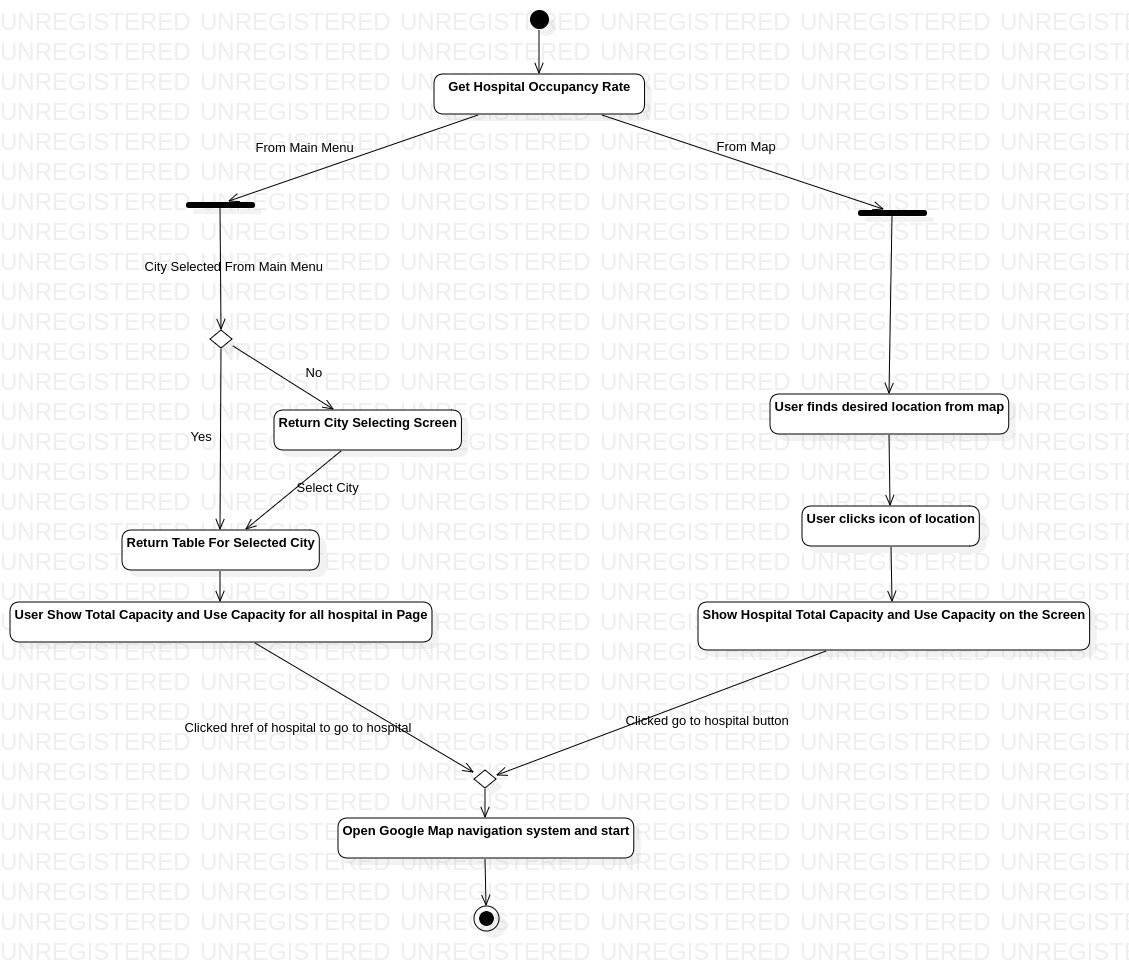
\includegraphics[scale = 0.4]{assets/ActivityDiagramSuggestion.jpg}
    \caption[Activity Diagram of Hospital Occupancy Rate]{Activity Diagram of Hospital Occupancy Rate}
\end{figure}

\section{Usability Requirements}
\begin{itemize}
    \item The mobile app should run on Android version 7.0+ since about 5 percent of android devices are still running on this version.
    \item The mobile app should run on IOS 15+ since 96\% of IOS users are using IOS 15 and 16.
    \item The mobile app should support PDF view for users to be able to see the PDF they Downloaded without any issues.
    \item Mobile app shall support accessibility modes on Android and IOS for users with disablities.
    \item Mobile app shall work in sync with AI assistants; Google Assistant, Siri and Bixby.
    \item Size of the app must be less than 10 megabytes, so that users can download it less than a minute.
\end{itemize}
\section{Performance Requirements}
\begin{itemize}
    \item Mobile app should start in 2 seconds after click, on a mid-level Android and old IOS device.
    \item Mobile app should cache datas to be able to show them during connection unstablities.
\end{itemize}
\section{Logical Database Requirements}
\begin{itemize}
    \item A local database should be created for mobile app to cache data.
    \item This database should contain all data available for a selected city.
\end{itemize}
\section{Design Constraints}
\begin{itemize}
    \item Mobile app should be designed in a way that it should not store, collect or send any inappropriate information about user.
    \item While app is being deleted, all data should be deleted to prevent data leak of users.
\end{itemize}
\section{System Attributes}
\subsection{Reliablity}
\begin{itemize}
    \item Fails on mobile application should be less than 5 seconds in 10 minutes of use.
    \item The app should crash at most once in 20 uses.
\end{itemize}

\subsection{Availability}
\begin{itemize}
    \item Users should be able to use old versions of app after updates for 30 days.
    \item App should be available for all 3 major operating systems; IpadOS, IOS, Android.
\end{itemize}

\subsection{Security}
\begin{itemize}
    \item App should be running in sandbox mode, ie. It should not reach any data on users device.
\end{itemize}

\section{Supporting Information}
All the APIs of afetbilgi.com, and the mobile app Afetbilgi, will be open source and free forever.